% Compile with xelatex (fontspec). Needs Comfortaa-Regular.ttf and
% Comfortaa-Bold.ttf next to this file, OR Comfortaa installed system-wide.
\documentclass[border=8pt]{standalone}
\usepackage{tikz}
\usepackage{fontspec}
\usetikzlibrary{arrows.meta,backgrounds,shapes.arrows,patterns}

\definecolor{wdgred}{HTML}{88171A}

% Opaque background: the logo must stay readable on dark pages (GitHub
% dark mode, admin dark theme), so white is baked into the SVG/PNG.
\pagecolor{white}

\newfontfamily\Comfortaa{Comfortaa}[
  Path = ./ ,
  UprightFont = Comfortaa-Regular.ttf ,
  BoldFont    = Comfortaa-Bold.ttf ]

\tikzset{
  lock/.pic={
    \draw[line width=1pt] (-0.1,0.1) arc (180:0:0.1);
    \draw[line width=1pt] (-0.1,0.1) -- (-0.1,0.05);
    \draw[line width=1pt] ( 0.1,0.1) -- ( 0.1,0.05);
    \fill[rounded corners=1pt] (-0.2,-0.12) rectangle (0.2,0.08);
    \fill[white] (0,0.0) circle (0.032);
    \fill[white] (-0.022,-0.07) rectangle (0.022,0.0);
  }
}

\begin{document}
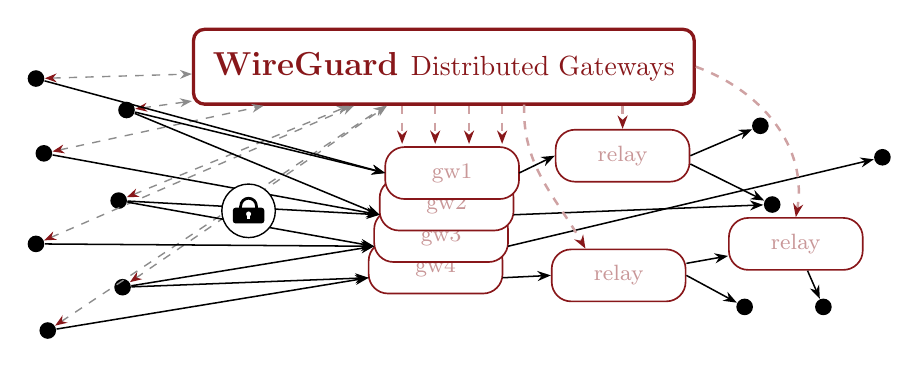
\begin{tikzpicture}[
    gw/.style    ={draw=wdgred, text=wdgred!45, line width=0.6pt, rounded corners=7pt,
                   fill=white, minimum width=1.7cm, minimum height=0.66cm},
    wgarrow/.style={draw=wdgred!40, line width=0.9pt, dashed,
                    -{Stealth[length=1.7mm, color=wdgred]}},
    wdg/.style   ={draw=wdgred, line width=1.2pt, rounded corners=4pt, fill=white,
                   text=wdgred, align=center, inner sep=7pt,
                   minimum width=4.9cm, minimum height=0.95cm},
    node2/.style ={circle, fill=black, inner sep=0pt, minimum size=6pt},
    ctrl/.style  ={draw=black!45, line width=0.5pt, dashed,
                   -{Stealth[length=1.5mm]}},
    data/.style  ={draw=black, line width=0.55pt, -{Stealth[length=1.7mm]}},
    exit/.style  ={draw=black, line width=0.55pt, -{Stealth[length=1.7mm]}},
  ]

  % ---- WordMark brick ----
  \node[wdg] (wdg) at (5.18,3.25)
      {\Comfortaa\large\bfseries WireGuard\ \mdseries\normalsize Distributed Gateways};

  % ---- red hatched arrow from WDG plunging through the stack ----

  % ---- vertical stack of gateways (overlapping); back -> front ----
  \node[gw] (g1) at (5.075,0.70){\footnotesize gw4};
  \node[gw] (g2) at (5.145,1.10){\footnotesize gw3};
  \node[gw] (g3) at (5.215,1.50){\footnotesize gw2};
  \node[gw] (g4) at (5.285,1.90){\footnotesize gw1};

  % four small parallel red arrows: WireGuard -> gateways
  \foreach \x in {4.65,5.07,5.50,5.92}{
    \draw[wgarrow] (\x,2.75) -- (\x,2.27); }

  % attach points on the exposed left/right band of each gateway
  \coordinate (L1) at (4.225,0.57);  \coordinate (R1) at (5.925,0.57);
  \coordinate (L2) at (4.295,0.97);  \coordinate (R2) at (5.995,0.97);
  \coordinate (L3) at (4.365,1.37);  \coordinate (R3) at (6.065,1.37);
  \coordinate (L4) at (4.435,1.90);  \coordinate (R4) at (6.135,1.90);

  % ---- clients (two columns, irregular) ----
  \node[node2] (c1) at (0.00,3.10){};
  \node[node2] (c2) at (1.15,2.70){};
  \node[node2] (c3) at (0.10,2.15){};
  \node[node2] (c4) at (1.05,1.55){};
  \node[node2] (c5) at (0.00,1.00){};
  \node[node2] (c6) at (1.10,0.45){};
  \node[node2] (c7) at (0.15,-0.10){};

  % ---- exits (irregular, far right): networks (dots) or relay gateways ----
  % NB: attach points are inverted vs labels: R4 = gw1 ... R1 = gw4.
  \node[node2] (e1) at (9.20,2.50){};
  \node[node2] (e2) at (9.35,1.50){};
  \node[node2] (e3) at (10.75,2.10){};
  \node[node2] (e4) at (9.00,0.20){};
  \node[node2] (e5) at (10.00,0.20){};
  \node[gw]    (relay)  at (7.40,0.60){\footnotesize relay};
  \node[gw]    (relay2) at (9.65,1.00){\footnotesize relay};
  \node[gw]    (relay3) at (7.45,2.12){\footnotesize relay};

  % control plane; the red chevron against each client marks the return leg
  \foreach \c in {c1,c2,c3,c4,c5,c6,c7}{
    \draw[ctrl, {Stealth[length=1.5mm, color=wdgred]}-{Stealth[length=1.5mm]}]
        (\c) -- (wdg); }

  % data plane: clients -> different gateways (encrypted)
  \draw[data] (c1) -- (L4);
  \draw[data] (c2) -- (L4);
  \draw[data] (c2) -- (L3);
  \draw[data] (c3) -- (L3);
  \draw[data] (c4) -- (L3);
  \draw[data] (c4) -- (L2);
  \draw[data] (c5) -- (L2);
  \draw[data] (c6) -- (L2);
  \draw[data] (c6) -- (L1);
  \draw[data] (c7) -- (L1);

  % exits: direct to a network, through one relay, or through two
  \draw[data] (R4) -- (relay3.west);     % gw1 -> relay3 -> e1, e2
  % start on the straight part of the east edge: the rounded corners make
  % TikZ's computed border point float off the visible outline
  \draw[exit] (relay3.east) -- (e1);
  \draw[exit] ([yshift=-3pt]relay3.east) -- (e2);
  \draw[exit] (R3) -- (e2);              % gw2 -> e2 (direct)
  \draw[exit] (R2) -- (e3);              % gw3 -> e3 (direct)
  \draw[data] (R1) -- (relay.west);      % gw4 -> relay -> e4
  \draw[exit] (relay.east) -- (e4);
  \draw[data] (relay) -- (relay2);       %        relay -> relay2 -> e5
  \draw[exit] (relay2) -- (e5);

  % the relays are driven by the control plane like any gateway
  \draw[wgarrow] (7.45,2.75) -- (relay3.north);
  \draw[wgarrow] (6.20,2.77) to[out=-92,in=120] ([xshift=-12pt]relay.north);
  \draw[wgarrow] (wdg.east) to[out=-20,in=80] (relay2.north);

  % padlock over the encrypted mesh
  \fill[white] (2.7,1.42) circle (0.34);
  \draw[black, line width=0.5pt] (2.7,1.42) circle (0.34);
  \pic at (2.7,1.38) {lock};

\end{tikzpicture}
\end{document}
